%%%%%%%%%%%%%%%%%%%%%%%%%%%%%%%%%%%%%%%%%%%%%%%%%%%%%%%%%%%%%%%%%%%%%%%%%%%%%%%%%%%%%%
%%%%%%%%%%%%%%%%%%%%  INGRESAR LAS PREGUNTAS DE LA  EVALUACIÓN %%%%%%%%%%%%%%%%%%%%%%%%
%%%%%%%%%%%%%%%%%%%%%%%%%%%%%%%%%%%%%%%%%%%%%%%%%%%%%%%%%%%%%%%%%%%%%%%%%%%%%%%%%%%%%%%

\paragraph{I} Read the following questions and identify the option that best answers each, then write ts letter on the line (5 points each)

\begin{preguntas}

\pregunta[5] \rule{1cm}{0.1mm} Select the option with a linear function:

\begin{enumerate*}[label=(\alph*)]
    \item $(a/b)x^2 + c\qquad$
    \item $\boxed{(a_1/b_1)x} \qquad$
    \item $(a/b)x^3 + c\qquad$
    \item $(a_n/b_n)x^2\qquad$
\end{enumerate*}

\pregunta[5] \rule{1cm}{0.1mm} Select the correct domain of $f(x):=\mathrm{abs}(x)$

\begin{enumerate*}[label=(\alph*)]
    \item $x\in\left(-\infty,0\right]\qquad$
    \item $x\in\left[-\infty,\infty\right]\qquad$
    \item $\boxed{x\in\left(-\infty,\infty\right)}\qquad$
    \item $x\in\left[0,\infty\right)\qquad$
\end{enumerate*}

\pregunta[5] \rule{1cm}{0.1mm} Select the option with the range of the function $f(x):=x^2$

\begin{enumerate*}[label=(\alph*)]
    \item $f(x)\in\left(-\infty,\infty\right)\qquad$
    \item $\boxed{f(x)\in\left[0,\infty\right)}\qquad$
    \item $f(x)\in\left(-\infty,0\right]\qquad$
    \item $f(x)\in\left[-1,1\right]\qquad$
\end{enumerate*}

\pregunta[5] \rule{1cm}{0.1mm} Select the option with the numeric value of the operation of functions, $f(x) + g(x)$, with $f(x):= x^2 + x$ and $g(x):=x+1$ at $x=2$,
%Select the correct type of function of $f(x):=x^n$, where $n\in\mathbb{Z}$ ($x$ belongs to the set of integer numbers

\begin{enumerate*}[label=(\alph*)]
    \item 18 $\qquad$
    \item 15 $\qquad$
    \item 12 $\qquad$
    \item \boxed{9} $\qquad$
\end{enumerate*}

\pregunta[5] \rule{1cm}{0.1mm} Select the alternative mathematical notation to express $f[g(x)]$

\begin{enumerate*}[label=(\alph*)]
    \item $\boxed{f\circ g}\qquad$
    \item $g\circ f\qquad$
    \item $f\to g\qquad$
    \item $f(g)\qquad$
\end{enumerate*}

\pregunta[5] \rule{1cm}{0.1mm} Select the option with the algebraic expression that shifts the linear function $f(x):=2x$, 5 units downward,
%Select the option of the function that map all the domain into the positive real numbers.

\begin{enumerate*}[label=(\alph*)]
    \item $f(x):=2(x+5)\qquad$
    \item $f(x):=2(x-5)\qquad$
    \item $f(x):=2x+5\qquad$
    \item $\boxed{f(x):=2x-5}\qquad$
\end{enumerate*}


\end{preguntas}

\newpage

\paragraph{II} Solve the following exercises in an orderly and clear manner. 
\textbf{Answers without procedure will not be considered.}
Underline or frame your final answer.

\begin{preguntas}

\pregunta[12] Tacking into account the following functions, 
\begin{gather*}
    f(x):=x+3,\quad g(x):=x+5,
\end{gather*}
express the algebraic representation of 
\begin{gather*}
    H(x):= g(x) + f(x).
\end{gather*}
%and evaluate the function $H(x)$ at $x=0$.

\begin{center}
    \framebox(0.9\textwidth,200){
    \begin{minipage}{\textwidth}
    \begin{align*}
        H(x) &= g(x) + f(x) \\
        &= (x+5) + (x+3) \\
        &= x+5 + x+3 \\
        &= 2x+8 \\
        &\boxed{H(x) = 2x+8}
    \end{align*}
    \end{minipage}
    }
\end{center}

\pregunta[12] Taking into account the following functions,
\begin{gather*}
    f(x):=\frac{4}{2}x,\quad g(x):=\frac{3}{6}x^2,
\end{gather*}
represent the algebraic expression of,
\begin{gather*}
    \frac{f(x)}{g(x)},\quad \frac{g(x)}{f(x)}.
\end{gather*}
%Finally, write the correct expression ($f(x)/g(x)$ or $g(x)/f(x)$) to get a linear function.

\begin{center}
    \framebox(0.9\textwidth,200){
    \begin{minipage}{0.45\textwidth}
        \begin{align*}
            \frac{f(x)}{g(x)} &= \left(\frac{4}{2}x\right)\left(\frac{6}{3}\frac{1}{x^2}\right) \\
            &= \cancelto{2}{\frac{4}{2}}\cancelto{2}{\frac{6}{3}}\frac{x}{x^2} \\
            &= 2\cdot 2\cdot x\cdot x^{-2} \\
            &= 4 x^{-1} \\
            & \boxed{\frac{f(x)}{g(x)} = 4 x^{-1} = \frac{4}{x}.}
        \end{align*}    
    \end{minipage}
    \begin{minipage}{0.45\textwidth}
        \begin{align*}
            \frac{g(x)}{f(x)} &= \left(\frac{3}{6}x^2\right)\left(\frac{2}{4}\frac{1}{x}\right) \\
            &= \cancelto{1/2}{\frac{3}{6}}\cancelto{1/2}{\frac{2}{4}}\frac{x}{x^2} \\
            &= \frac{1}{2}\cdot \frac{1}{2}\cdot x^{2}\cdot x^{-1} \\
            &= \frac{1}{4} x \\
            & \boxed{\frac{f(x)}{g(x)} = \frac{1}{4} x.}
        \end{align*}
    \end{minipage}
    }
\end{center}

\newpage

\pregunta[18] Sketch the following functions

\begin{enumerate*}[label=(\alph*)]
    \item $g(x):= \mathrm{abs}(x)-1\qquad$
    \item $h(x):= \mathrm{abs}(x-1)\qquad$
\end{enumerate*}

\begin{figure}[ht!]
    \centering
    \begin{subfigure}[c]{0.45\textwidth}
        \centering
        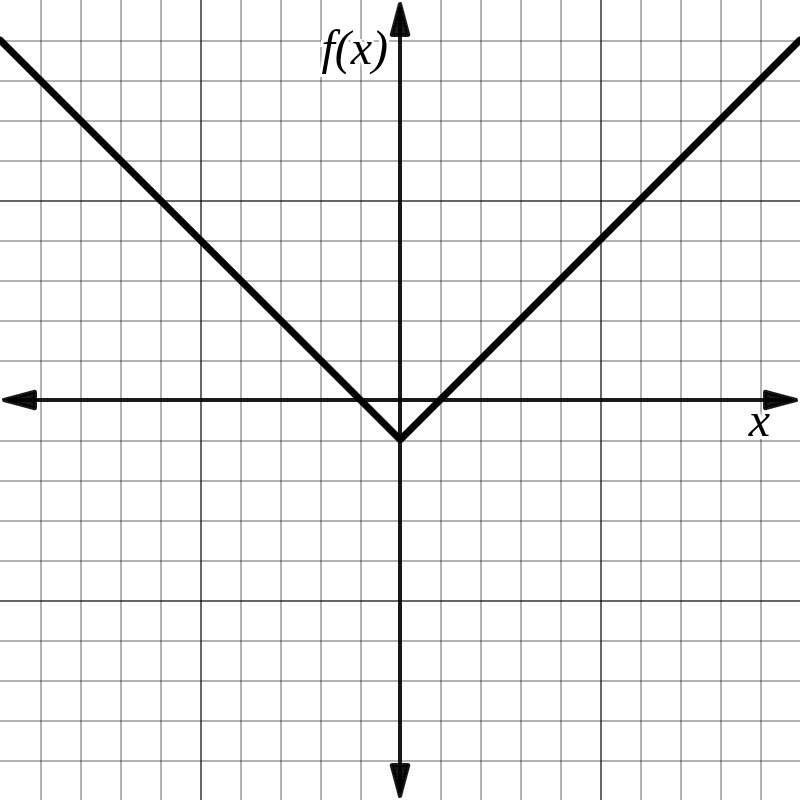
\includegraphics[width=\textwidth]{NO TOCAR/imagenes/absy_1.png}
        \caption{~}
    \end{subfigure}
    \begin{subfigure}[c]{0.45\textwidth}
        \centering
        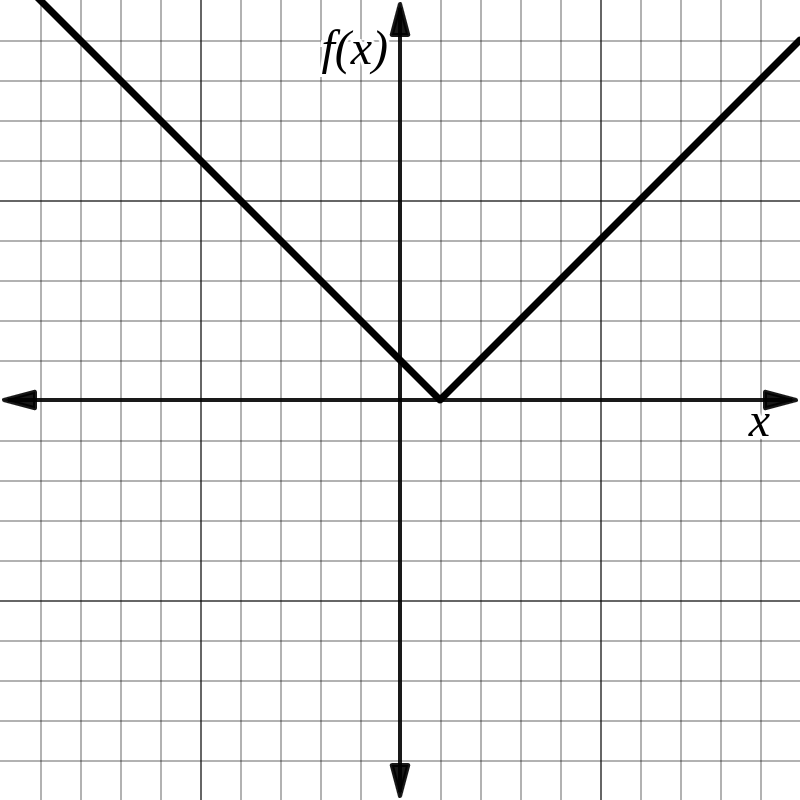
\includegraphics[width=\textwidth]{NO TOCAR/imagenes/absx_1.png}
        \caption{~}
    \end{subfigure}

   %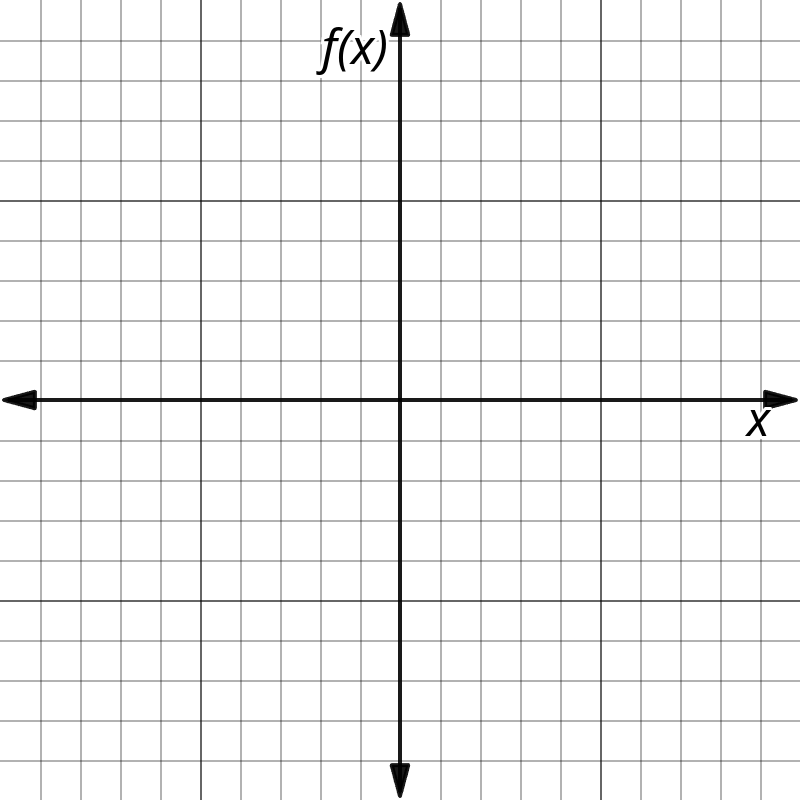
\includegraphics[width=0.7\textwidth]{NO TOCAR/imagenes/cartesian-plane.png}
\end{figure}


and write the translation between $f(x):= \mathrm{abs}(x)$ with $g(x)$ and $f(x):= \mathrm{abs}(x)$ with $h(x)$,

\begin{center}
    \framebox(0.9\textwidth,150){
    \begin{minipage}{0.85\textwidth}
     The function $g(x)$ has a downward shift with respect the function $f(x)$.
    On the other hand, the function $h(x)$ has a lateral shift to the right with respect $f(x)$. 
    \end{minipage}
    }
\end{center}


\pregunta[12] Express the algebraic expression and the domain of $(f\circ g)(x)$ with $f(x):=\sqrt{x}$ and $g(x):=x^2$.
%Write the type of function for each graph (linear, cubic,absolute value, quadratic), % Change the order
\begin{center}
    \framebox(0.9\textwidth,150){
    \begin{minipage}{\textwidth}
        \begin{align*}
            (f\circ g)(x) &= \sqrt{x^2} \\
            &= (x^2)^{1/2} \\
            &= x^{2\frac{1}{2}} \\
            &= x \\
            & \boxed{(f\circ g)(x) = x,\quad x\in(-\infty,\infty)}
        \end{align*}
    \end{minipage}
    }
\end{center}



\begin{comment}
\begin{figure}[ht!]
    \centering
    \begin{subfigure}[c]{0.45\textwidth}
        \centering   
        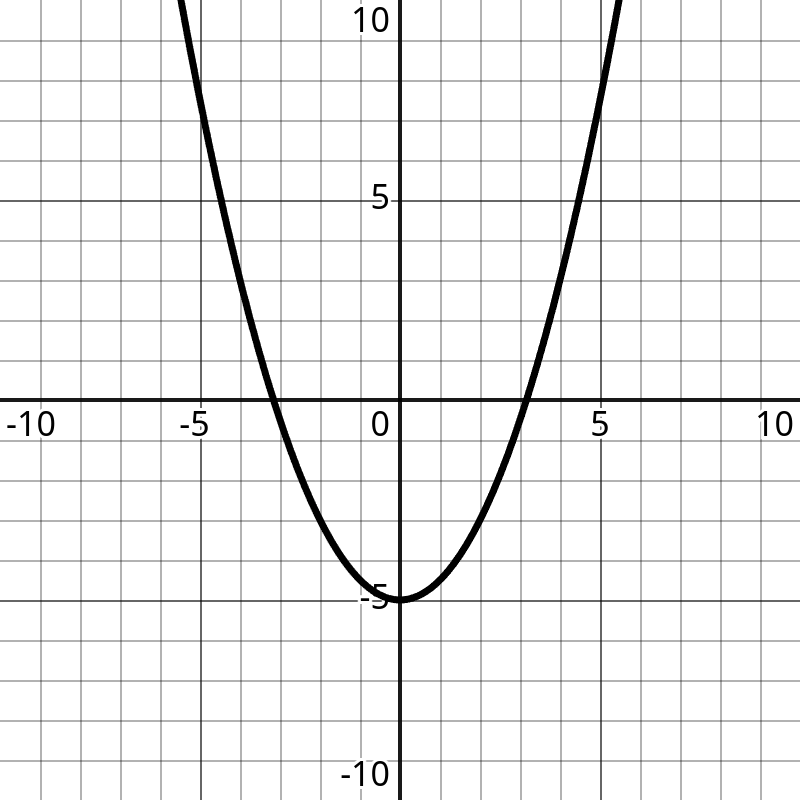
\includegraphics[width=0.75\textwidth]{NO TOCAR/imagenes/cuadratic.png}
    \end{subfigure}
    \begin{subfigure}[c]{0.45\textwidth}
         \centering
         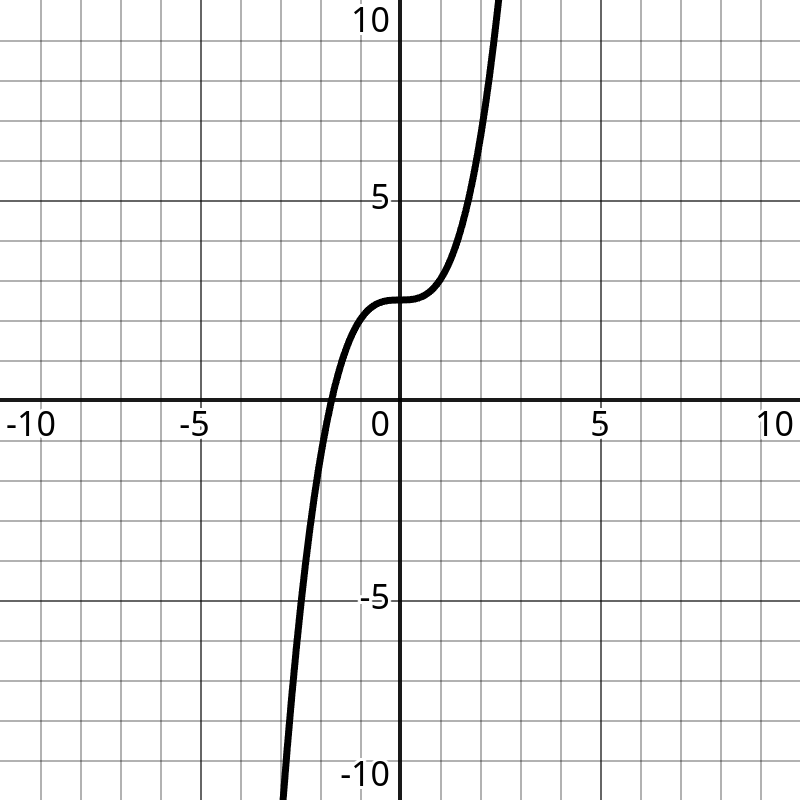
\includegraphics[width=0.75\textwidth]{NO TOCAR/imagenes/cubic.png}
    \end{subfigure}
    
    \vspace{1.5cm}

    \begin{subfigure}[c]{0.45\textwidth}
         \centering
         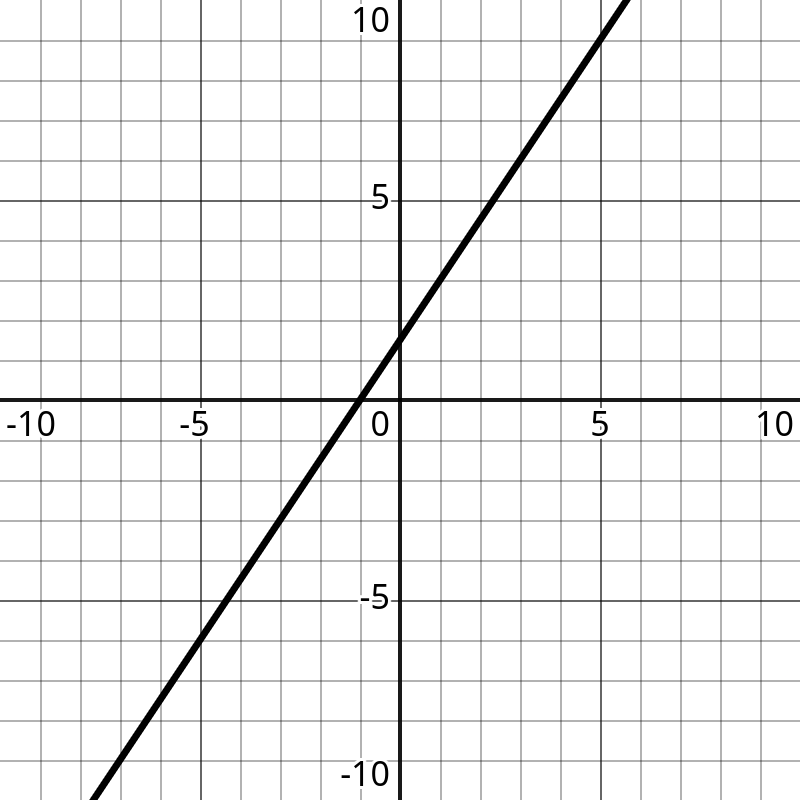
\includegraphics[width=0.75\textwidth]{NO TOCAR/imagenes/linear.png}
    \end{subfigure}
    \begin{subfigure}[c]{0.45\textwidth}
        \centering
        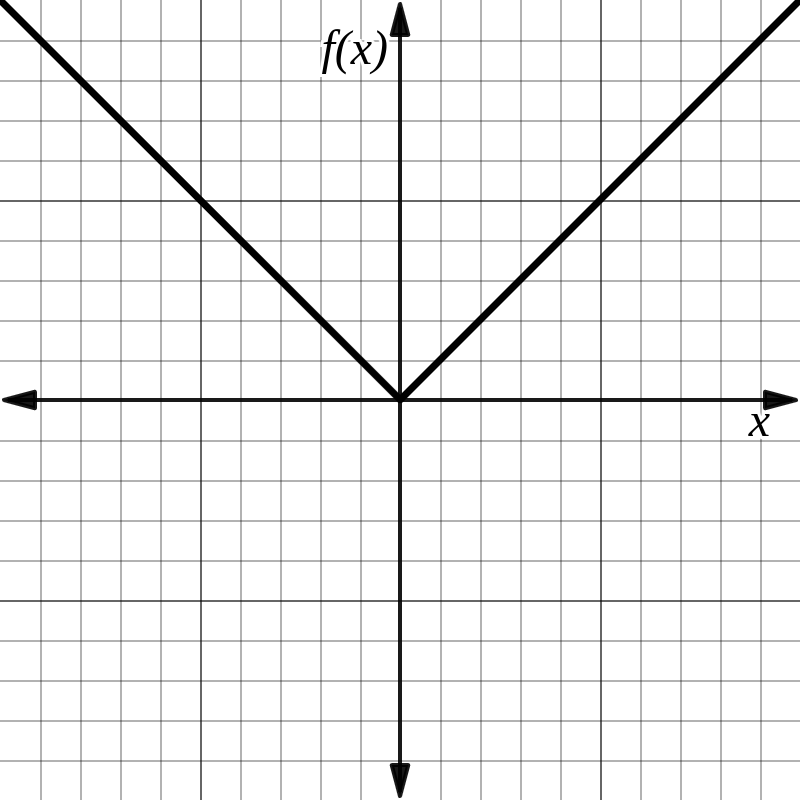
\includegraphics[width=0.75\textwidth]{NO TOCAR/imagenes/abs.png}
    \end{subfigure}
\end{figure}
\end{comment}

\newpage

\pregunta[6] Reduce algebraically the following operation with $f(x)=x-1$ and $g(x)=x-1$,
\begin{gather*}
    f(x) \times g(x)
\end{gather*}
%Graph a sketch of the following function,

\begin{center}
    \framebox(0.9\textwidth,200){
    \begin{minipage}{0.85\textwidth}
        \begin{align*}
            f(x)g(x) &= (x-1)(x-1) \\
                     &= x^2 -x -x + 1 \\
                     &= x^2 -2x +1 \\
                     & \boxed{f(x)g(x) = x^2 -2x +1}
        \end{align*}
    \end{minipage}
    }   
\end{center}

\begin{comment}
 \begin{figure}[ht!]
    \centering
    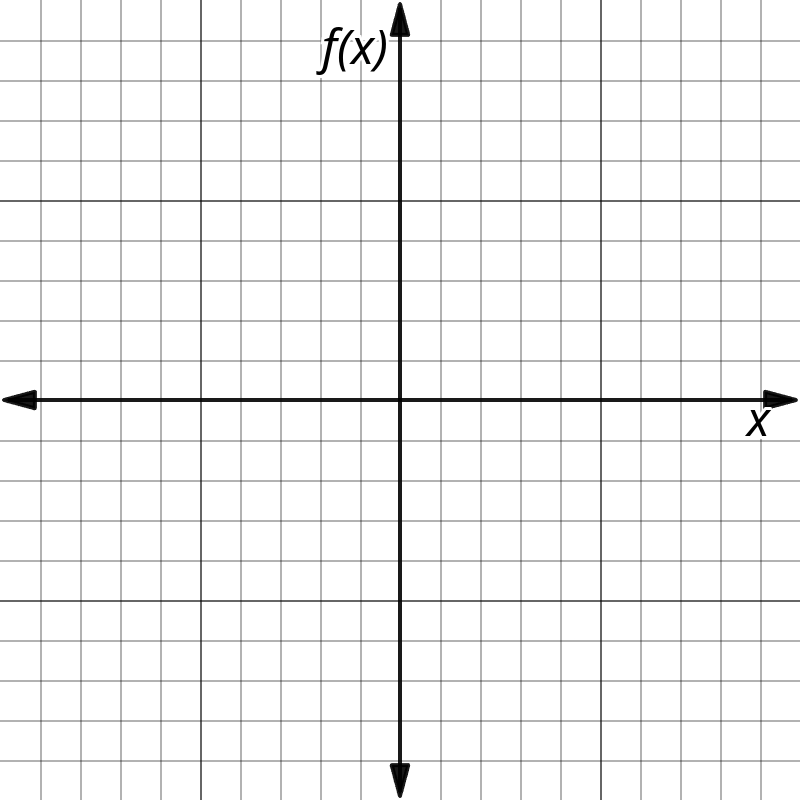
\includegraphics[width=0.7\textwidth]{NO TOCAR/imagenes/cartesian-plane.png}
\end{figure}
\end{comment}


\pregunta[10] Suppose that $H(x):=\sqrt{x+1}+2(x+1)^2$. Find two functions $f(x)$ and $g(x)$ such that $H(x):=(f\circ g)(x)$

\begin{center}
    \framebox(0.9\textwidth,350){
    \begin{minipage}{0.85\textwidth}
    Taking into account that
    \begin{gather*}
        H(x) = \sqrt{x+1} + 2(x+1)^2,
    \end{gather*}   
    we can introduce the following change of variable, $a=x+1$,
    \begin{gather*}
        H(x) = \sqrt{a} + 2(a)^2,
    \end{gather*}
    this function can de redefined as: $f(a)=\sqrt{a} + 2a^2$.
    If we change $a$ for $x$, we get,
    \begin{gather*}
        \boxed{f(x)=\sqrt{x}+2x^2.}
    \end{gather*}

    Now, from the change of variable $a=x+1$, we can defined a function $g(x)$,
    \begin{gather*}
        \boxed{g(x) = x+1.}
    \end{gather*}

    Finally, to see that does definitions works, we carry on the composition of functions,
    \begin{align*}
        (f\circ g)(x) &= (\sqrt{x}+2x^2 \circ x+1)(x) \\
        &= \sqrt{x+1}+2(x+1)^2
    \end{align*}
    
    \end{minipage}
    }
\end{center}


\end{preguntas}

